\documentclass{report}
\title{Thesis proposal}
\author{Yannick Hold-Geoffroy  \\
    Universit\'e laval  \\
    }

\date{\today}


\usepackage[utf8]{inputenc}
\usepackage{times}
\usepackage{amsmath}
\usepackage{amssymb}
\usepackage{cite}   % sort citation numbers automatically
\usepackage{url}
\usepackage{graphicx}
\usepackage{rotating}
%\usepackage{authblk}
% to control spacing in item lists
\usepackage{enumitem}
\usepackage[pagebackref=false,breaklinks=true,colorlinks,bookmarks=false]{hyperref}


% Hint: \title{what ever}, \author{who care} and \date{when ever} could stand 
% before or after the \begin{document} command 
% BUT the \maketitle command MUST come AFTER the \begin{document} command! 
\begin{document} 

\maketitle

\tableofcontents

% Commands
\newcommand{\boldomega}{\boldsymbol \omega} % bold omega
\newcommand{\boldmu}{\boldsymbol \mu} % bold omega
\newcommand{\bolddelta}{\boldsymbol \delta} % bold delta

\graphicspath{{figures/}}

%\begin{abstract}
%\end{abstract}


\chapter*{Symbols and notations}

\begin{table}[htbp]\caption{Symboles et notations}
\centering % to have the caption near the table
\begin{tabular}{r c p{10cm} }

\hline & & \\
$\langle \cdot, \cdot \rangle$      & $=$ & Scalar (dot) product \\
$\bold{x}$                          & $=$ & Vector \\
$X$                                 & $=$ & Matrix \\
$\omega$                            & $=$ & Angle \\
\hline
\end{tabular}
\label{tab:TableOfNotationForMyResearch}
\end{table}


%%%%%%%%%%%%%%%%%%%%%%%%%%%%%%%%%%%%%%%%%%%%%%%%%%%%%%%%%%%%%%%%%%%%%%%%%%%%%%%%
\chapter{Introduction}

%Comment la numérisation du monde est à nos portes et c'est le futur.
%La reconstruction 3d est un sujet de plus en plus présent dans la vie de tous les jours.

%Reconstruction 3D extérieure à large échelle.

%Utilisations: Jeux vidéos, préserver la culture, réalité augmentée, diffusion


\section{Photometric Stereo}

Décrire la PS, ses entrées, ses sorties, ses forces (1 normale par px), ses faiblesses, citer Woodham.

%La Stéréoscopie Photométrique (SP) est une technique permettant de récupérer la structure d'une scène à partir d'indices photométriques. Elle donne en sortie une carte de normale. Cette carte définie, pour chaque pixel de l'image, la normale de la surface correspondante dans la scène. Une fois la carte de normale obtenue, il est possible de l'intégrer afin d'obtenir un maillage 3d de la surface.

%Pour fonctionner, la PS a besoin d'une séquence d'images en entrée.

Dans sa forme de base, la SP...

\cite{Woodham1979}

\begin{equation}
\bold{b} = \rho L(\mathbf{\boldomega}) \langle \boldomega, {\bf n} \rangle \,,
\end{equation}

\begin{figure}
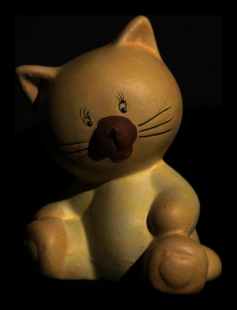
\includegraphics[width=.1\linewidth]{PS/cat_0.png}
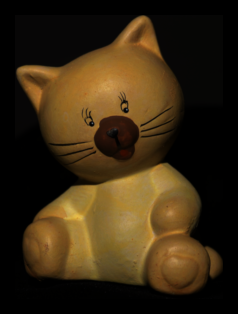
\includegraphics[width=.1\linewidth]{PS/cat_3.png}
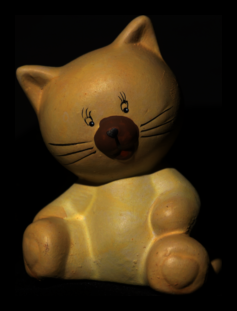
\includegraphics[width=.1\linewidth]{PS/cat_4.png}
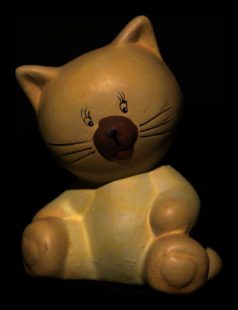
\includegraphics[width=.1\linewidth]{PS/cat_5.png}
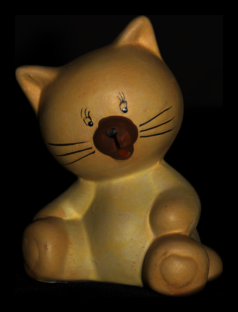
\includegraphics[width=.1\linewidth]{PS/cat_10.png}
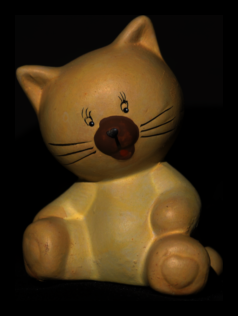
\includegraphics[width=.1\linewidth]{PS/cat_11.png}

\includegraphics[width=.1\linewidth]{PS/cat_normal_map.png}
\caption{Exemples d'images d'entrée. 	
Images from CSE 455, 2010 by Neel Joshi, Ira Kemelmacher and Ian Simon}
\label{fig:PS_example}
\end{figure}

PS was confined to the lab until recently.

Illumination incontrôlable, coplanarité du soleil.

In this thesis [...]


%%%%%%%%%%%%%%%%%%%%%%%%%%%%%%%%%%%%%%%%%%%%%%%%%%%%%%%%%%%%%%%%%%%%%%%%%%%%%%%%
\chapter{State of the Art Review}

% Expliquer les améliorations de la PS au travers du temps:
% \begin{itemize}
% 	\item Unknown lighting
% 	\item Unknown BRDF
% 	\item Robustness
% 	\item Outdoor (algorithme et analyse)
% 	\begin{itemize}
% 		\item Yu
% 		\item Boxin shi
% 	\end{itemize}
% \end{itemize}

Since its inception in 1979, PS has received a lot of attention throughout the years. Researchers tried to alleviate the restrictive assumptions of the original method, such as lambertian reflectance, noiseless sensors and known lighting. This chapter will first relate the major improvements made on PS over the years, and then focus on the efforts made to bring it outside the laboratory.

\section{Photometric Stereo}

% Ackermann
% Basri
% ...
\cite{basri-ijcv-2007,BarskyPetrou-pami-2003,alldrin-cvpr-08,ikehata-cvpr-12,ikehata-cvpr-14}.

As previously stated, PS has been studied extensively for many decades. Covering the vast amount of work done is beyond the scope of this thesis proposal. The rest of the document will focus more closely on work that have considered PS on outdoor conditions.

\section{Outdoor Photometric Stereo}

% webcams
The first works attempting PS reconstruction on outdoor data~\cite{ackermann-cvpr-12,abrams-eccv-12} made the observation that, over the course of a day, the sun seems to move on a planar path through the sky. Unfortunately, co-planar light sources yield an under-constrained, two-source PS problem~\cite{hernandez-pami-11}, which cannot be solved without strong regularization and reconstruction artifacts. To avoid this issue, the authors therefore propose gathering months of data using webcams.
% PLS -- Merge with pervious
To tackle this new challenge, a natural first strategy has been to experiment with Lambertian reflectance and to model the sun as a point light source, to match a well-studied lab condition. Unfortunately, approaches based on this model have practical limitations caused by the movement of the sun in the sky for a given day. Depending on the latitude and time of year, its trajectory may lie too close to a plane~\cite{shen-pg-14}, yielding an under-constrained, two-source PS problem~\cite{hernandez-pami-11}. Possible solutions include waiting for a day when the sun trajectory is non-planar~\cite{shen-pg-14}, or capturing several months of data~\cite{ackermann-cvpr-12,abrams-eccv-12} to ensure good conditioning. 

% single day
Recently, Shen~{\em et al.}~\cite{shen-pg-14} showed that, contrary to common belief, the sun path in the sky actually does not always lie within a plane. Thus, PS reconstruction can sometimes be computed in a single day even with a point light source model. The main downside of this approach is that planarity of the sun path (\ie, conditioning of PS reconstruction) depends on the latitude and the time of year. More specifically, reconstruction becomes unstable at high latitudes near the winter solstice, and worldwide near the equinoxes.

% richer lighting models
To compensate for limited sun motion, other approaches have proposed using richer models of illumination that account for additional atmospheric factors in the sky. Typically, this is done by employing (hemi-)spherical environment maps~\cite{debevec-siggraph-98}. On one hand, full environment maps can be captured and used with calibrated PS algorithms~\cite{yu-iccp-13,shi-3dv-14,hung-wacv-15}. On the other hand, it is also possible to estimate part of the environment map without explicitly capturing it, by synthesizing a hemispherical model of the sky using physically-based models~\cite{inose-tcva-13,jung-cvpr-15}. While these richer models do allow reconstructions from only one day, it is unknown whether the same could be done with even less data. 

% hold-geoffroy
The work presented below extends our initial analysis in~\cite{holdgeoffroy-iccp-15}. Rather than presenting a new reconstruction algorithm, in~\cite{holdgeoffroy-iccp-15} we conducted an empirical analysis of the same sky database to identify which days provide more favorable atmospheric conditions for outdoor PS. However, no consideration was given to the shortest time interval of data capture needed to obtain accurate reconstructions; all results were reported on at least 6 hours (a ``full day'') of captured data. Here, instead of comparing days, we focus on analyzing different time intervals within each day. We then show that 6 hours is actually more than necessary, and detail the relationship between the appearance of the sky hemisphere and the quality of PS reconstruction.

% nishino -- single image
Finally, it is also worth mentioning shape-from-shading techniques such as~\cite{oxholm-eccv-12,johnson-cvpr-11,barron-pami-15} [Add Horn?], which push reconstruction to its limits by attempting to recover shape from a single input image. In this case, the information provided by the shading cue is obviously insufficient to define a unique solution, so these approaches rely strongly on priors of different types and complexities. In this paper, we avoid such strong priors and focus our analysis exclusively on the photometric/shading cues obtained from multiple images. 




%%%%%%%%%%%%%%%%%%%%%%%%%%%%%%%%%%%%%%%%%%%%%%%%%%%%%%%%%%%%%%%%%%%%%%%%%%%%%%%%
\chapter{Existing contributions}

Philosophie: big-data

\section{HDR database}

Décrire le Mean Light Vector, décrire notre base de données de ciels, décrire comment on peut appliquer la philosophie Big Data à ce problème.

\section{What Is a Good Day for Outdoor Photometric Stereo?}

% From ICCP
A promising approach to answer this question is to use more elaborate models of illumination---high dynamic range (HDR) environment maps~\cite{reinhard-book-05}---as input to outdoor PS. Promising results have been reported in~\cite{yu-iccp-13} for outdoor images taken within an interval of just eight hours (in a single day). However, the quality of outdoor results is reported to be inferior to that obtained in indoor environments, the decline being attributed to modest variation in sunlight. This observation leads to an interesting, yet unanswered question: had the sun path and atmosphere conditions been different on that day, could the quality of their results have been better? Or, in other words: what makes it a good day for outdoor Photometric Stereo? 

As one might expect, the answer to the question above is intrinsically tied to the orientation of a particular surface patch, the associated hemisphere of lighting directions observed by the patch, and the variation in lighting intensity in that hemisphere over the course of a day. So far, this question has only been explored in laboratory conditions or with simple directional illumination, where optimal lighting configurations can be theoretically derived~\cite{drbohlav-iccv-05,klaudiny-prl-14,shen-pg-14}. No attempt has been made at answering this question with more realistic illumination models in an outdoor setup, where lighting cannot be controlled and atmospheric effects are difficult to predict.

In this paper, we present a systematic analysis of the expected performance of photometric stereo algorithms in outdoor settings. To explore the influence of these effects, we exploit a large database of outdoor HDR environment maps, which provides a rich sampling of the variability in outdoor illumination. Through a theoretical analysis (inspired by \cite{sun-ivc-07}) and supported by an extensive empirical evaluation as well as a preliminary quantitative validation, we derive confidence intervals that allow us to predict when surface normals can be reconstructed more accurately and solely from the photometric cue. Instead of focusing exclusively on sun position~\cite{shen-pg-14}, our analysis incorporates the influence of all components of natural lighting: sun, sky, clouds, etc., as well as noise and surface albedo. 

This paper does \emph{not} introduce a novel photometric stereo algorithm. Rather, we explore the conditions in which PS may or may not work, when faced with the challenging case of uncontrollable outdoor illumination. Our main goal is to provide guidance for future research by assessing the \emph{reconstructibility} of surface patches as a function of their orientation and the illumination conditions, given a set of HDR environment maps captured throughout a single day.

% Assumptions
To make this novel analysis tractable, we make the following assumptions. We consider Lambertian surface patches, and assume that at most one day of data can be used. We also assume that the dominant part of the light comes from the sky hemisphere (sun, sky, clouds, etc.) and surface patches are independent (cast shadows and inter-reflections are not modeled).


\section{$x$-hour Outdoor Photometric Stereo}
3DV15


%%%%%%%%%%%%%%%%%%%%%%%%%%%%%%%%%%%%%%%%%%%%%%%%%%%%%%%%%%%%%%%%%%%%%%%%%%%%%%%%
\chapter{Proposed contributions}

% Metho!

\begin{equation}
b_t = \frac{\rho}{\pi} \int_{\Omega_{\bf n}} L_t(\mathbf{\boldomega}) \langle \boldomega, {\bf n} \rangle d\omega \,,
\end{equation}

\section{Calibrated outdoor reconstruction}

\section{Blind outdoor reconstruction}

\section{Emploi d'autres astres que le soleil}

Décrire le projet day \& night.

\section{Augmentation avec d'autres techniques}

% from ICCP
While these techniques can lead to well-defined solutions, they are not always practical in many scenarios with strict temporal or geographical constraints. A second strategy has therefore been to combine PS with other techniques such as multi-view stereo~\cite{inose-tcva-13,shi-3dv-14}, or use reference objects as in \cite{johnson-cvpr-11} or example-based PS~\cite{hertzmann-pami-05,ackermann-3dv-14}. But can we accurately reconstruct surface geometry simply based on the photometric cue in an outdoor setting, without overly restrictive temporal and geographical constraints?

Décrire l'amélioration que pourrait apporter la PS utilisée conjointement avec du SFM et la stéréo multivues standard.


%%%%%%%%%%%%%%%%%%%%%%%%%%%%%%%%%%%%%%%%%%%%%%%%%%%%%%%%%%%%%%%%%%%%%%%%%%%%%%%%
\chapter{Échéancier}

\begin{itemize}
	\item 2016h: Selection and Calibrated PS algorithm
	\item 2016e: Capture, Blind PS algorithm  
	\item 2016a: Blind PS algorithm, Day \& night
	\item 2017h: Fusion with SFM
	\item 2017e: Capture, Fusion with Multiview Stereo Techniques
	\item 2017a: 
	\item 2018h: Écrire et soutenir.
\end{itemize}


%%%%%%%%%%%%%%%%%%%%%%%%%%%%%%%%%%%%%%%%%%%%%%%%%%%%%%%%%%%%%%%%%%%%%%%%%%%%%%%%
\chapter{Conclusion}\label{conclusion}

Recap.

{\small
%\bibliographystyle{ieee}
\bibliography{main}
}

\end{document}
